\pagenumbering{arabic}

\chapter{Images and Videos}

\section{Definitions}
\subsection{Computer Vision}
Is the science and technology of machines that see, where “see” means that the machine is able to extract information from an image that is necessary to solve some task. The image data can take many forms, such as video sequences, views from multiple cameras, or multidimensional data from a medical scanner.

Some examples of applications of computer vision include systems for controlling processes, like an industrial robot or an autonomous vehicle, detecting events as for visual surveillance or people counting, or again organizing information for example for indexing databases of images and image sequences, even modeling objects or environments like in industrial inspection, medical image analysis or topographical modeling and interaction as the input to a device for computer-human interaction.

\begin{figure}[h]
    \centering
    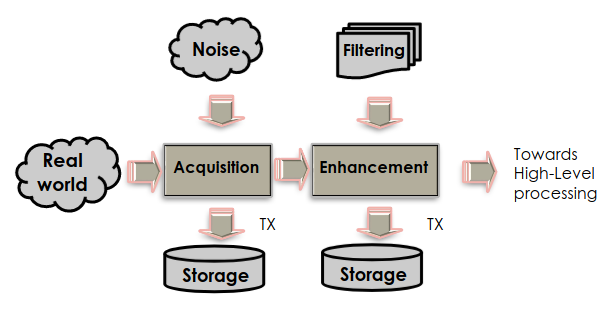
\includegraphics[scale=0.5]{Figures/ProcessingChain.png}
    \caption{The processing chain(The first part is more about signal and video, in this course we'll focus mainly on the second half)}
    \label{fig:enter-label}
\end{figure}

\subsection{Acquisition}
It refers to the process of transferring a portion of the real 3D world onto a 2D surface bringing a continuous-parameter real world into a discrete-parameter one. 
The acquisition process is the first step in the processing chain and it is the transformation of a physical signal into an electrical one, by means of a sensor. 
Remember that the sensor is a device that responds to a physical stimulus (light, heat, pressure, etc.) and produces an electrical signal. 
\textit{PS: The representation is in a standard format.}
\\
\subsection{Digital Images}
A digital image is a representation of a two-dimensional image as a finite set of digital values, called picture elements or pixels. The digital image contains a fixed number of rows and columns of pixels, it's a collection of coordinates. Pixels are the smallest individual element in an image, a single pixel represents a projection of a portion of the real world, holding quantized values that represent the brightness of a given color at any specific point. Pixels can be \textbf{Grayscale} or \textbf{Color}. 
Grayscale images are represented by a single component, typically 8bit, while color images are represented by three components, typically 24bits.
\\
\subsection{Sampling}
Is the process of converting a continuous signal into a discrete signal. This is because the "real world" is a continuous function, while computers are digital. Analog video is a 1-D continuous function where one spatial dimension is mapped onto time by means of a scanning process, while digital video is instead sampled in a three dimensions (2D spatial and 1D temporal).
\\
\begin{figure}[h]
    \centering
    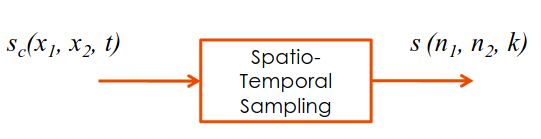
\includegraphics[scale=0.5]{Figures/Sampling.png}
    \caption{Sampling}
    \label{fig:enter-label}
\end{figure}

\textit{In a Nutshell:}
\begin{itemize}
    \item Continuous signal \[ s_c(x_1, x_2)\]
    \item Spatial rectangular sampling \[ x_1 = n_1 \bigtriangleup x_1, x_2 = n_2 \bigtriangleup x_2\]
    \item So \[ s(n_1, n_2) = s_c(n_1 \bigtriangleup x_1, n_2 \bigtriangleup x_2)\]
    \item Once we have the digital format, we can manipulate data and apply filters, change colors, store and transmit.
\end{itemize}

For what concerns handling images we need only to know that pixels are numbered starting from the top left corner (so the top left corner is the origin, arrow down for the rows and right for the columns).
The value of a pixel in a certain position is defined as \(I(r,c)\), where \(r\) is the row index and \(c\) the column one. (Start at 0 or 1, depends on you :D)
Monochrome images have values normalized in the range \([0,1]\), where 0 is black, 1 is white and the intensity is called \textit{grey level}. While color pictures have 3 channels (RGB) and the values are normalized in the same way.
\section{Color}
But what is color? It's the attribute the human visual system associates to objects, more scientifically, it's a mathematical relationship that combines different wavelengths. 
It's important to check whether something we see is what we expect, to recognize objects or to distinguish similar things. For example, a white car, that for us is obviously white, for a computer is a combination of red, green and blue, moreover it has some black points for the wires, some point gray due to the street, etc.
\\For this reason we need to talk about color perception. The human eye is like a camera with a focal length of about 20mm, where the iris controls the amount of light by adjusting the size of the pupil. 
The perception of color is possible through cones in the fovea that has around 100M receptors.  Cones have peak responses on three main wavelengths, red (700nm), green (546.1nm) and blue (435.8nm).
\\
But going back to the main topic, data can be processed locally but even transmitted remotely or archived on a storage unit. The problem is that images and videos require a lot of bandwidth, so we need to compress them with a codec.
A codec is a device or computer program for encoding or decoding a digital data stream or signal in the compressed domain. It stands for coder-decoder, and it's a way to reduce the dimension of the file (e.g JPEG, MPEG, DIVX). 
\\It is important to mention that compression is lossy, so reduces quality (we lose some information) and can even introduce visual artifacts such as blocking, blurring, chromatic aberrations(plus some noise from the sensor). However, the loss is not a problem because the human visual system is not perfect.
\\\textit{NB1: There exists even lossless compression, but it's not used much.
\\NB2: Processing is typically done in the uncompressed domain.}
\\To make a final comparison, raw images are usually stored in a 1D vector of pixels, while compressed images reduce the dimension of the file with or without loss of information.

\subsection{Additive color model}
The additive color model is a method to create color by mixing the primary colors.
\begin{figure}[h]
    \centering
    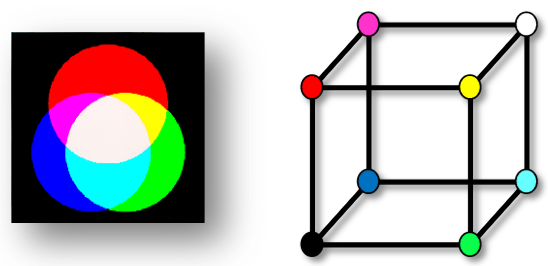
\includegraphics[scale=0.5]{Figures/AdditiveModel.png}
    \caption{Additive Color Model}
    \label{fig:enter-label}
\end{figure}
\\
Colored beams are projected onto a black surface, then overlap so the human eye receives the stimula without generating interference, mixing the components and perceiving the resulting color.
Starting from the primary colors RGB we can obtain:
\begin{multicols}{2}
    \begin{itemize}
        \item R+G = Yellow
        \item R+B = Magenta
    \end{itemize} 
    \columnbreak
    \begin{itemize}
        \item B+G = Cyan
        \item R+G+B = White
    \end{itemize}
\end{multicols}
\textit{NB: Subtractive color is the inverse process.}\\
Looking at the image above we can identify the gray scale along the diagonal connecting the black corner with the white corner.
\\
About the way colors combined, we can have:\\
\begin{tabular}{p{0.5\textwidth} p{0.5\textwidth}}
    \begin{itemize}
        \item White: RGB(1,1,1)
        \item Black: RGB(0,0,0)
        \item Gray: RGB(0.5,0.5,0.5)
    \end{itemize}
    &
    \begin{itemize}
        \item Green: RGB(0,1,0)
        \item Yellow: RGB(1,1,0)
    \end{itemize}
\end{tabular}
\\When we take a colored image and separate it into its three RGB components, we notice that these components are correlated. This means that the grayscale versions of the individual RGB channels contain almost the same amount of information. 
Among these, the green component has a stronger response compared to the red and blue components. Additionally, the human eye is more sensitive to variations in luminance and contrast than to color differences. 
Therefore, using a different representation might be more effective for certain applications.
An example could be the YCbCr color space, where Y, the luminance is separated from Cb and Cr that are the chrominance.
Or again the HSV, where H is the hue (color), S is the saturation (brightness) and V is the value (intensity).
\\\textit{PS: YCbCr is a generalization of YUV, just a matter of conversion matrices (Downsampling).}

\begin{figure}[h]
    \begin{subfigure}{0.5\textwidth}
        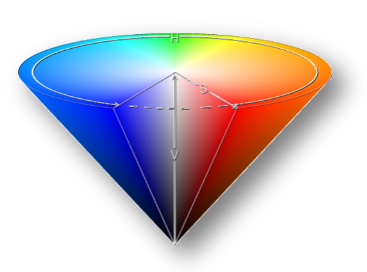
\includegraphics[scale=0.4]{Figures/HSV1.png} 
        \label{fig:subim1}
    \end{subfigure}
    \begin{subfigure}{0.5\textwidth}
        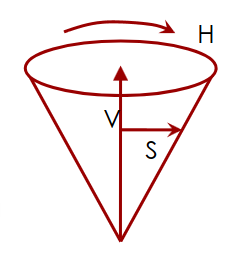
\includegraphics[scale=0.5]{Figures/HSV2.png}
        \label{fig:subim2}
    \end{subfigure}
        
        \caption{HSV Color Space}
        \label{fig:image2}
\end{figure}

Summing up just a little bit:
\begin{itemize}
    \item RGB is used in general for visualization, in displays each pixel in composed by three phosphors (CRT) or LEDs (LCD);
    \item YUV is suitable for compression since we are less sensitive to chrominance variations and U and V can be downsampled;
    \item HSV is robust for computer graphics and image analysis.
\end{itemize}

\subsection{Bayer Pattern}
In the acquisition phase, light is captured by the CCD (Charge Coupled Device) that is an array of cells. Each cell is a photosensitive element that converts light into an electrical signal.
The Bayer pattern is a color filter array for arranging RGB color filters on a square grid of photosensors. The best solution would be to have devices with 3 different CCDs and to correctly exploit the human eye response there would be three types of photosensors of color filters 50\% green, 25\% red and 25\% blue.
\\\textit{NB: Green sensors are defined as luminance-sensitive elements, while the red and blue ones are defined as chrominance-sensitive.}
\subsection{Quantization}
Like in the mono-dimensional case, signals need to be quantized. That implies the definition of a number of levels to define our signal. Typically, the range 0-1 is quantized using 8bpp but even other representations with 10-12 bpp are available.
But why 8bpp? Well, 8bpp represent 256 levels, which is fine for the human eye, that can distinguish 100 levels of grey. Indeed, if we quantize with less that 6bpp (64 levels, minimum to ensure smooth pictures), then false contours will appear $\Rightarrow$ contouring.
\subsection{Limits of the 2D}
Images provide reliable information about static scenes.
We lose motion information like temporal evolution of the scene, rapid changes, dynamics of motion (qualitative and quantitative) and even how subjects/objects relate one to each other.
Moreover, analyzing a video provides a more consistent representation of the scene.
It’s closer to what humans do every day.

\subsection{Video}
A video is a sequence of 2D images that represent a projection of moving 3D scene onto the video camera image plane. It's expected that adjacent frames are strongly correlated.
For what concerns the resolution, the images are up to 50mp, while in video is typically lower, $4$k is $3840\times2160=8.3$mp, $8$k is $7680\times4320=33.2$mp and full HD is around $2$mp.
The reasons are that video can last hours, so we need to store a lot of data, and that the human eye is less sensitive to resolution in motion. 
Just to move on a little bit, when analyzing an image, key features of interest include color distribution and the presence of edges and contours, which help identify and define objects.

In the context of video analysis, additional benefits emerge. Consistency of features over time allows for tracking object movement, while changes in the scene can reveal dynamic interactions. Videos also enable the detection of objects entering or exiting the frame.

Several factors contribute to the complexity of scene analysis. These include the presence of multiple objects, occlusions, shadows, noise, motion, illumination changes, clutter, and non-rigid objects. Each of these elements introduces challenges that require sophisticated techniques to accurately interpret the scene.
\subsection{Histogram}
The histogram is a simple way to describe the color distribution of a picture, indeed, it can be seen as a probability density function and it represents the occurrence of all colors on a graph.
In other words it’s a statistical representation of the pixel values. For an $M \times N$ image
\[
    hist(p) = \frac{I(x,y)}{M \times N}
\]
Where $I(x,y)$ is the intensity of the pixel at position (x,y) and $M \times N$ is the total number of pixels in the image.\\
The equation holds for one component, so in case of more components, a histogram can be obtained from each of them.
\begin{figure}[h]
    \centering
    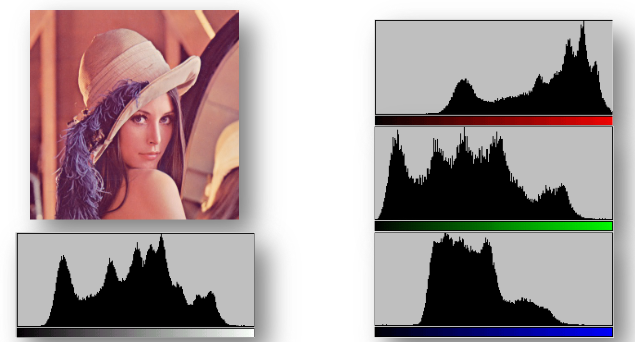
\includegraphics[scale=0.5]{Figures/Histogram.png}
    \caption{Histograms of Lana}
    \label{fig:enter-label}
\end{figure}
\\
A histogram provides valuable insights into various aspects of an image. It can reveal whether the image is dark or bright by showing the distribution of pixel intensities. 
Additionally, it indicates whether colors are distributed equally or if there are dominant or missing colors.
\\
Applications of histogram analysis are diverse. 
In environmental monitoring, histograms help assess whether the illumination of a scene is appropriate. 
By comparing histograms over time, one can detect changes in the background, such as in the past two hours. 
Moreover, histograms can assist in object identification by determining whether the observed moving object matches the characteristics of object A or B. 
\\Overall, a histogram serves as a "signature" that can be applied across various domains for image analysis and interpretation.
\subsection{Operations}

\textbf{Stretching:}
\\Is a simple operation to change the dynamic range of the image by stretching the histogram and increasing the contrast by applying a piecewise linear function. 
\begin{figure}[h]
    \centering
    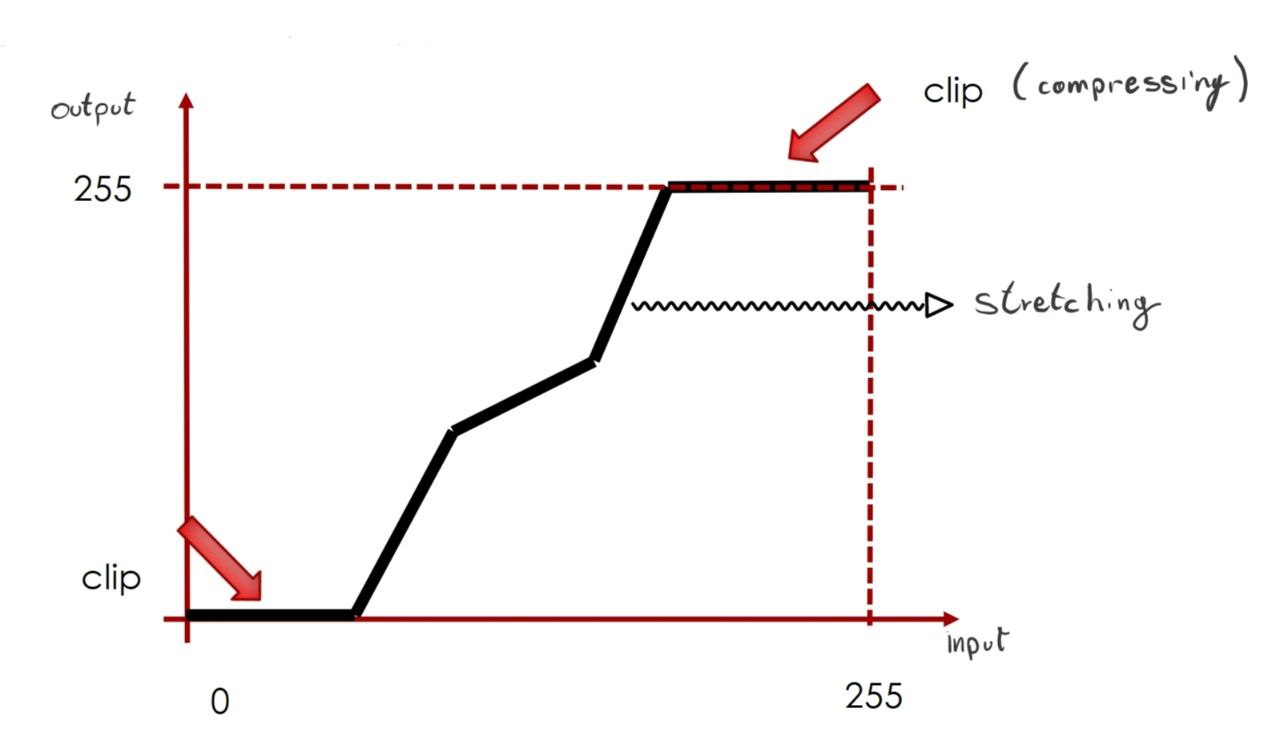
\includegraphics[scale=0.3]{Figures/Stretching.jpeg}
    \caption{Stretching}
    \label{fig:enter-label}
\end{figure}   
\\ 
\textbf{Equalization:}
\\Working on the statistics of the pixels it is possible to improve the quality of an image. Ideally we’d like to obtain a FLAT histogram, and to do so we have to compute the cumulative histogram (equivalent to CDF).
Basically, we compute the sum of all bins, then we subtract the minimum value and normalize the result by dividing for the number of pixels minus 1.
Notice that this operation can introduce artifact, indeed, looking at the image, we can notice that some bins are empty. Concerning the visual final aspect, the image is more contrasted (similarly to stretching), but the noise is enhanced.
    \[
        CHist_I(p) = \sum_{k=0}^{p} hist(k)
    \]
    \[
        hist_eq(p) = \frac{CHist(p)-CHist_{min}}{M \times N-1}\times 255
    \]
\begin{figure}[h]
    \centering
    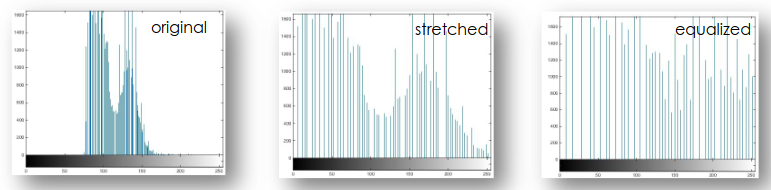
\includegraphics[scale=0.5]{Figures/OperationsHist.png}
    \caption{Different operations on the histogram}
    \label{fig:enter-label}
\end{figure}
    
\section{Edge extraction}
We perceive objects primarily through their color (appearance model) and shape. Shape, defined by the boundary between an object and the rest of the image, is crucial for object recognition. A sharp change in image brightness often indicates an edge, highlighting these boundaries.
\\
However, environmental conditions like cast shadows or surface orientation can affect these perceptions, causing changes in appearance. Additionally, edges might not always be meaningful, especially in textured areas or when noise is present. These factors can complicate the task of recognizing objects based on their shape and edges alone.
\\Steps:
\begin{itemize}
    \item Determine intensity, and possibly the direction of an edge for each pixel location through gradient or Laplacian;
    \item Find a threshold and binarize.
\end{itemize}
\textit{NB: The first step is the most difficult one. Different tools are available, but we’ll focus here on the gradient-based algorithms.}
\\\\
\textbf{Edge extraction by gradient analysis}\\
As for mono-dimensional signals, the goal is to find maxima and minima but, differently from the 1D case, here we also have a direction. This means finding a gradient along a line $r$ oriented in the direction $\theta$.
\[
\frac{\partial f}{\partial r} = \frac{\partial f}{\partial x}\frac{\partial x}{\partial r} + \frac{\partial f}{\partial y} \frac{\partial y}{\partial r} = f_x \cos(\theta) + f_y \sin(\theta)
\]
\\
The edge extraction process consists of computing the 1st order derivative in two orthogonal directions, $f_1$ and $f_2$. To each of them we associate an amplitude.
Going a little more into the concrete, for edge detection typically we use FIR filters, that are linear and shift-invariant. The most common are the Prewitt, Roberts and Sobel operators.
\\
For the first two we have to choose a convolution mask and apply it to the picture. The convolution is computed for both masks and a threshold is chosen to highlight only the strongest edges.
\\
\textbf{Roberts operator:} $\begin{bmatrix} 1 & 0 \\ 0 & -1 \end{bmatrix} \quad \begin{bmatrix} 0 & 1 \\ -1 & 0 \end{bmatrix}$
\vspace{0.5cm} 
\textbf{Prewitt operator:} $\begin{bmatrix} -1 & 0 & 1 \\ -1 & 0 & 1 \\ -1 & 0 & 1 \end{bmatrix} \quad \begin{bmatrix} -1 & -1 & -1 \\ 0 & 0 & 0 \\ 1 & 1 & 1 \end{bmatrix}$
\\
\textit{NB: The Prewitt operator is preferred because it is isotropic $\Rightarrow$ you know where is the center.}
\\
For the Sobel operator, we have to apply two masks, one for each orthogonal direction. The mask is a 3x3 matrix and the gradient is computed for each point. Then we have to threshold the result by doing the square root of the sum of the squares of the two gradients.
This because Sobel tends to introduce a lot of noise, so we need to smooth the result.
\\\vspace{1cm} 
\textbf{Sobel operator:} $D_x=\begin{bmatrix} -1 & 0 & 1 \\ -2 & 0 & 2 \\ -1 & 0 & 1 \end{bmatrix} \quad D_y=\begin{bmatrix} -1 & -2 & -1 \\ 0 & 0 & 0 \\ 1 & 2 & 1 \end{bmatrix}$
\\
The convolution with the FIR masks is performed similarly to the 1D convolution. Take the mask, rotate, slide from left to right and associate to the central point the value of the convolution. 
\\What you're going to see is the convolution expressed in 2D, in which we have to deal with two components, x and y.
\\\textit{NB: We know that a convolution in space has a counterpart in frequency in forms of multiplication.}
\\ In space: \[ g(x,y)= f(x,y)*h(x,y) \]
In frequency: \[ G(u,v)= F(u,v) \cdot H(u,v) \]
\\
\[ y(m,n)= x(m,n)*h(m,n) = \sum_{m'=-\infty}^{\infty} \sum_{n'=-\infty}^{\infty} h(m-m',n-n') \cdot x(m',n')\]
From a practical point of view, we rotate the mask by 180° and then we keep shifting it on the image. The result of the multiplication of coefficients and pixel values will be stored in the output image in the application point (the central one).
\begin{figure}[h]
    \centering
    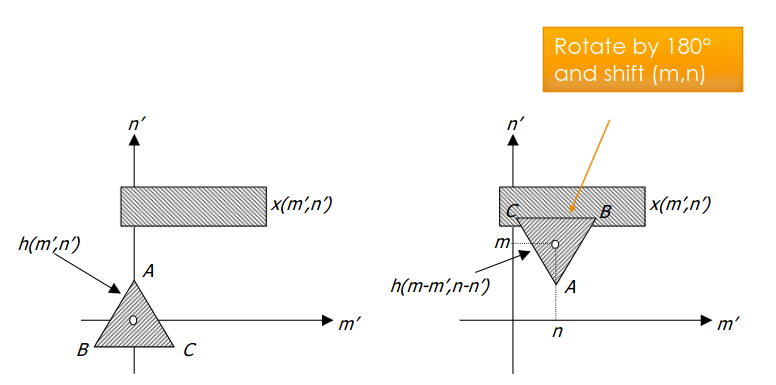
\includegraphics[scale=0.3]{Figures/Convolution.png}
    \caption{How to (convolution edition)}
    \label{fig:enter-label}
\end{figure}

\section{Filters}
Now we are going to see some filters that are using as smoothing or enhancing operators.
\subsection{Low-pass filtering}
Low-pass is the easiest filter and it basically consists of averaging the values in the sliding window. The window is a matrix of size $m \times n$ and the result is obviously the average of the values in the window.
\[
    I_{LP}(x,y) = \frac{1}{mn} \sum_{x=-a}^{a} \sum_{y=-b}^{b} I(x,y)
\]
It preserves low-frequency components and removes the high-frequency ones. It's a sorta of weighted sum of low high frequency functions. So, it cuts the high frequency components above the threshold and smooths the image. 
\\Average filtering $\Rightarrow$ average of the pixels in the window $\Rightarrow$ bigger the filter, more the smoothing (the difference is smaller). It also helps denoising the signal. 

\subsection{Gaussian filtering}
Gaussian filtering is a low-pass filter used to remove high-frequency components from an image, effectively blurring it and reducing noise. 
It operates as a 2D convolution filter that employs a Gaussian function, which is isotropic and does not require flipping the mask. 
The mask, centered in the middle, is sized to ensure integer values. 
Using a Gaussian mask is advantageous because, in the Fourier domain, it remains a Gaussian. 
This symmetry and lack of rotation simplify the convolution process.
\[
    G(x,y) = \frac{1}{2\pi\sigma^2}e^{-\frac{x^2+y^2}{2\sigma^2}}
\]
\textit{NB: The bigger, the better. The central pixels are more considered, far pixels have a lower impact.}
\subsection{Median filtering}
\begin{figure}[h]
    \centering
    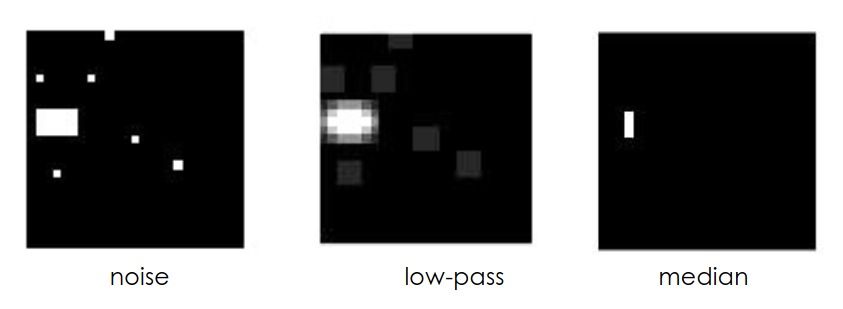
\includegraphics[scale=0.5]{Figures/Noise.png}
    \label{fig:enter-label}
\end{figure}
Median filtering is a nonlinear technique used to remove noise from an image. This spatial domain method replaces each pixel value with the median value of its surrounding neighborhood pixels. 
It is especially effective for removing salt and pepper noise and is ideal for images corrupted by impulse noise.
\\
While smoothing techniques work well for zero-mean noise, they are less effective for handling spikes, as low-pass (LP) filtering tends to blur the noise, spreading it and creating artifacts. 
Median filtering avoids this issue by not relying on convolution. 
Instead, it sorts the pixel values in the filter's neighborhood and assigns the median value to the central pixel. 
This approach prevents the noise from spreading, although it may leave some noise if the filter size is too small. On the other hand, bigger size can introduce artifacts.
\section{Morphology}

Morphology refers to the study of the shape of regions in an image, focusing on operations that assess and manipulate these shapes. The goal is to determine if one shape fits into another, detect holes of specific sizes, or remove areas smaller than a threshold\dots 
\\It involves non-linear filtering using a structuring element, which is a predefined arbitrary shape. This element slides over the image, comparing its pattern with the image at each position.
\\
There are four main operations: Erosion, Dilation, Opening and Closing.\\
Erosion and Dilation are self-explanatory, the first one reduces the area of a shape, the second one enlarges it. Instead, opening and closing are a combination of erosion and dilation. Opening gets rid of small portions of the image close to the boundaries of relevant areas, while closing fills holes and makes region boundaries smoother. 
\\\textit{Concerning structuring elements, depending on the type of shape we want to edit, the right element must be chosen.}
\subsection{Dilation}
\begin{figure}[h]
    \centering
    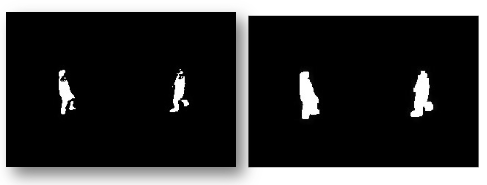
\includegraphics[scale=0.5]{Figures/Dilatation.png}
    \caption{Dilation}
    \label{fig:enter-label}
\end{figure}
Dilation is a morphological operation that is used to enlarge the boundaries of regions of foreground pixels in an image. It is used to merge the objects in the image. The structuring element is a binary mask that defines the neighborhood of the pixel. The dilation of the image is obtained by sliding the structuring element over the image and placing the origin of the structuring element at the center of the pixel. 
\\More formally, the dilation of an image $B$ by a structuring element $S$ is given by:
\[
    B \oplus S = \cup_{b \in B} S_b
\]
Sweep the structuring element on the whole image, as the origin of the structuring element touches a “1” of the image all pixels of the structuring element are OR’ed to the output image. 
\\\textit{PS: OR/union $\Rightarrow$ every time that the structuring element touches a 1, the output is 1, so it enlarges the shape.}
\subsection{Erosion}
\begin{figure}[h]
    \centering
    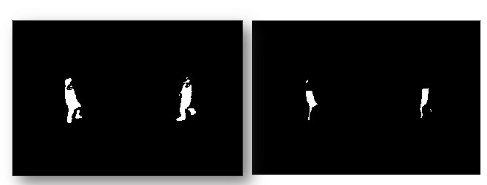
\includegraphics[scale=0.5]{Figures/Erosion.png}
    \caption{Erosion}
    \label{fig:enter-label}
\end{figure}
Erosion is a morphological operation that is used to reduce the boundaries of regions of foreground pixels in an image. It is used to separate the objects in an image.
Sweep the structuring element on the whole image, at each position where every 1-pixel of the structuring element covers a 1-pixel of the binary image, the binary image corresponding to the origin is OR’ed with the output image (the pixel is set to 1). 
\\More formally, the erosion of an image $B$ by a structuring element $S$ is given by:
\[
    B \ominus S = \{b | b + S \in B \quad \forall s \in S\} 
\]
Erosion of A by B can be understood as the locus of points reached by the center of B when B moves inside A.
\\
\textit{NB: If before it was enough for the center to touch a 1, now ALL must touch a 1. All the structuring element must be contained in the image.}
\subsection{Closing and Opening}
\begin{figure}[H]
    \centering
    \begin{minipage}[b]{0.45\textwidth}
        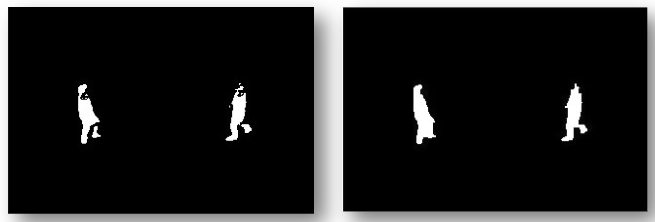
\includegraphics[scale=0.3]{Figures/Closing.png}
        \caption{Closing}
    \end{minipage}
    \begin{minipage}[b]{0.45\textwidth}
        \begin{itemize}
            \item Closing \\ $\Rightarrow$ first dilate and then erode; \\ Non-contiguous regions are first merged, then the boundaries are refined.
        \end{itemize}
    \end{minipage}
    
    \vspace{1cm} 
    
    \begin{minipage}[b]{0.45\textwidth}
        \begin{itemize}
            \item Opening \\ $\Rightarrow$ first erode and then dilate; \\ First small areas are removed, then residual information is refined.
        \end{itemize}
    \end{minipage}
    \begin{minipage}[b]{0.45\textwidth}
        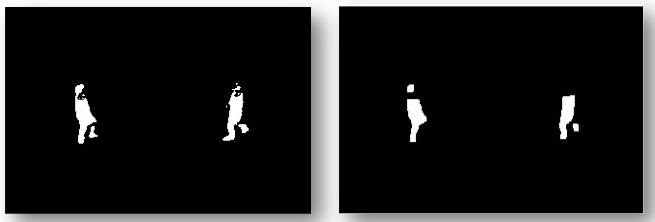
\includegraphics[scale=0.3]{Figures/Opening.png}
        \caption{Opening}
    \end{minipage}
\end{figure}

These operations are in general non-reversible, so the result depends on the order of the operations.
